\documentclass[border=2pt, 10pt]{standalone}

\usepackage{fontspec}
    \setmainfont{Times New Roman}

\usepackage[dvipsnames]{xcolor}
    \definecolor{GDLcolor}{HTML}{A6A6A6}
    \definecolor{ELcolor}{HTML}{E8E490}

\usepackage{tikz}
    \usetikzlibrary{math}
\usepackage{siunitx}

\begin{document}
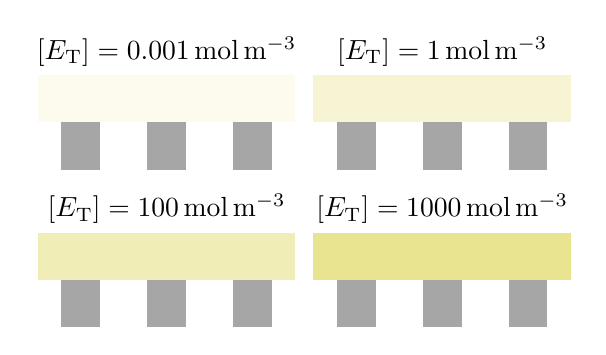
\begin{tikzpicture}

    \tikzset{%
        pics/ET/.style args={#1/#2}{%
                code={%

                        \tikzmath{%
                            \dpore=0.6;
                            \epsilonGDL=0.55;
                            \deltawall=(1-\epsilonGDL)*\dpore/\epsilonGDL;
                            \deltafig=3*\dpore+3*\deltawall;
                            \deltaGDL=0.6;
                            \deltaEL=0.6;
                        };

                        \fill [ELcolor, opacity=#1] (0, 0) rectangle (\deltafig, \deltaEL);
                        \foreach \i in {0, ..., 2} {%
                                \fill [GDLcolor] ({\dpore/2+\i*(\deltawall+\dpore)}, 0) rectangle ++(\deltawall, -\deltaGDL);
                            }
                        \node at (\deltafig/2, 0.9) {\ensuremath{
                                [E_\mathrm{T}] = \qty{#2}{\mole \per\cubic\meter}
                            }
                        };

                    }
            }
    }

    \pic at (0, 0) {ET=0.15/0.001};
    \pic at (3.5, 0) {ET=0.4/1};
    \pic at (0, -2) {ET=0.65/100};
    \pic at (3.5, -2) {ET=1/1000};

\end{tikzpicture}
\end{document}